% -*- mode:LaTex; mode:visual-line; mode:flyspell; fill-column:75-*-

\chapter{In-Situ Self-Pose Estimation for Modular Continuum Robots}
\label{chapLimbs}

Continuum robots have gained attention for their compliance and adaptability compared to rigid-link robots, enabling safe interaction and smooth, continuous deformation inspired by biological structures such as octopus arms and elephant trunks ~\cite{russo2023continuum}. These traits support dexterous manipulation and navigation in confined or cluttered spaces, making continuum robots well suited for search and rescue ~\cite{yamauchi2022development}, minimally invasive surgery ~\cite{burgner2015continuum}, inspection ~\cite{wang2021design}, and human--robot interaction ~\cite{abah2021multi}.

\begin{figure}[!t]
\centering
    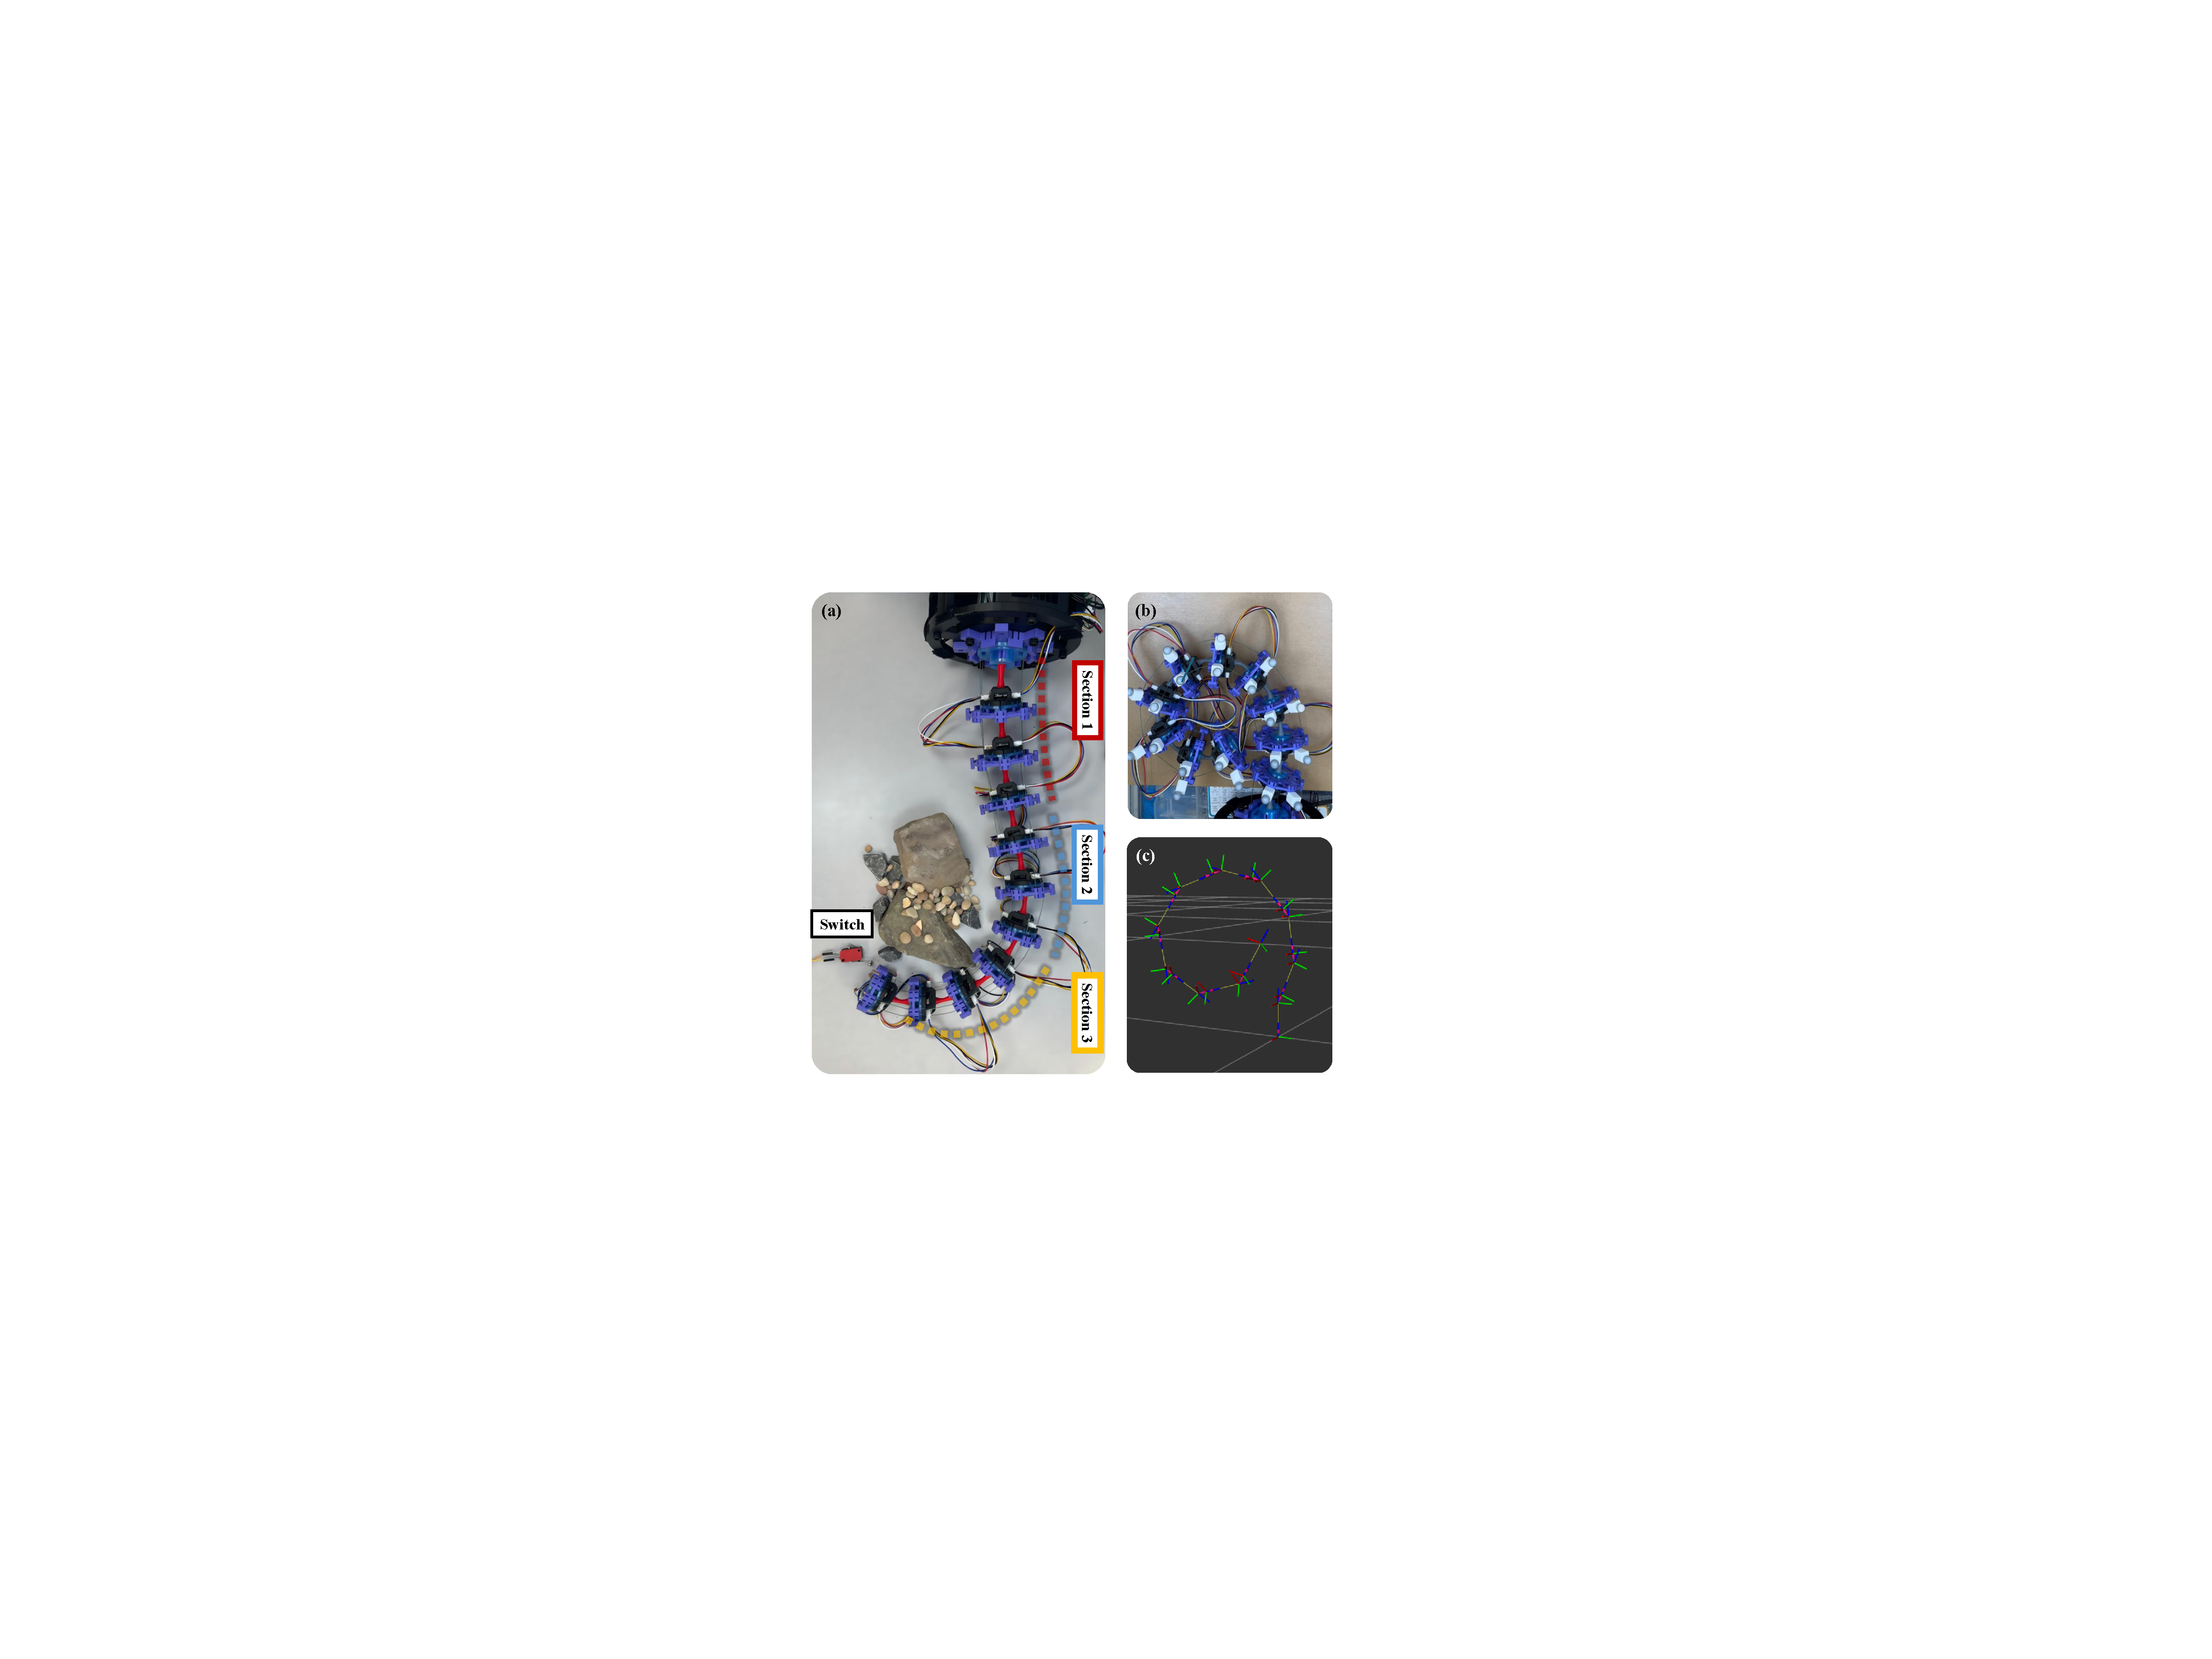
\includegraphics[totalheight=13cm]{figs/limb/Fig1_v3.pdf}
    \caption{(a) Example of the proposed modular continuum robotic platform. In this example, a 10-segment robot with joints of high (Section 1), medium (Section 2), and low (Section 3) stiffness is used to produce a shape that can reach around an obstacle and contact a switch. (b) Example of a large-deformation configuration of the robot under rotational motion. (c) Corresponding pose estimation result for the configuration shown in (b).}
    \label{fig:overall}
\end{figure}

Most existing continuum robots are still task-specific and built in an ad hoc way, with fixed geometry, actuation, and mechanical properties that are difficult to reconfigure. As a result, adapting them to new tasks often requires major redesign and refabrication, limiting scalability and broader adoption. This lack of modularity stands in contrast to the versatility that continuum robots are theoretically capable of providing.

Other major barriers to the practical deployment of continuum robots are sensing and state estimation. Unlike rigid robots with a small set of joint variables, continuum robots have effectively infinite degrees of freedom, making shape and pose estimation difficult. Many existing approaches therefore rely on external infrastructure such as motion capture systems, cameras, or tracking rigs ~\cite{sincak2024sensing, lu2023image}. While these methods are effective in laboratory environments, they increase cost and complexity and limit deployment outside controlled settings.

To address these limitations, this chapter presents a self-contained modular continuum robotic platform that combines mechanical reconfigurability with embedded proprioceptive sensing. The system is designed around modular continuum joints that can be rapidly assembled, replaced, or reconfigured to meet different task requirements without sacrificing the smooth shape morphing and compliance that make continuum robots attractive. The mechanical behavior of each joint is programmable through interchangeable elements with precomputed stiffness characteristics, enabling users to specify desired robot shapes and deformation profiles in a principled manner.

Beyond mechanical modularity, the platform enables self-pose estimation with onboard sensing, avoiding external tracking. We use magnetic sensing to infer each joint's configuration and adopt a modular inference pipeline in which sensing is performed at the joint level and then combined across the full robot. The system is experimentally validated in grasping and traversal tasks, demonstrating both mechanical adaptability and effective self-sensing without external pose feedback during operation.

In summary, the main contributions of this chapter are as follows:
\begin{enumerate}
    \item The design of a modular, reconfigurable continuum robotic platform.
    \item A method for programming robot shape through interchangeable joints with precomputed stiffness properties.
    \item A self-contained pose estimation approach using magnetic sensing with a modular joint-level sensing pipeline.
    \item Experimental validation of the proposed system in traversal, pose-estimation, and grasping tasks.
\end{enumerate}

\section{Modular Design}

\subsection{Modular Design and Fabrication}

Modularity is a central feature of the proposed continuum robot platform. The robot, shown in Fig.~\ref{fig:structure}, comprises identical rigid core segments that are 3D printed in carbon-fiber-reinforced PET and connected by compliant 3D-printed TPU joints. Each core segment houses the electronics for pose estimation and includes dovetail features for joint attachment, as well as outer slots for interchangeable PLA rings whose diameter and geometry can be customized for specific applications. These rings can also accept task-specific accessories, for example high-friction studs for gripping.

This architecture supports an arbitrary number of segments, limited primarily by tendon actuation. In this study, 8- and 10-segment robots actuated by servo-driven tendons were used to demonstrate variable joint stiffness and the resulting sensing and control performance in representative grasping tasks.

\begin{figure*}[!t]
\centering
    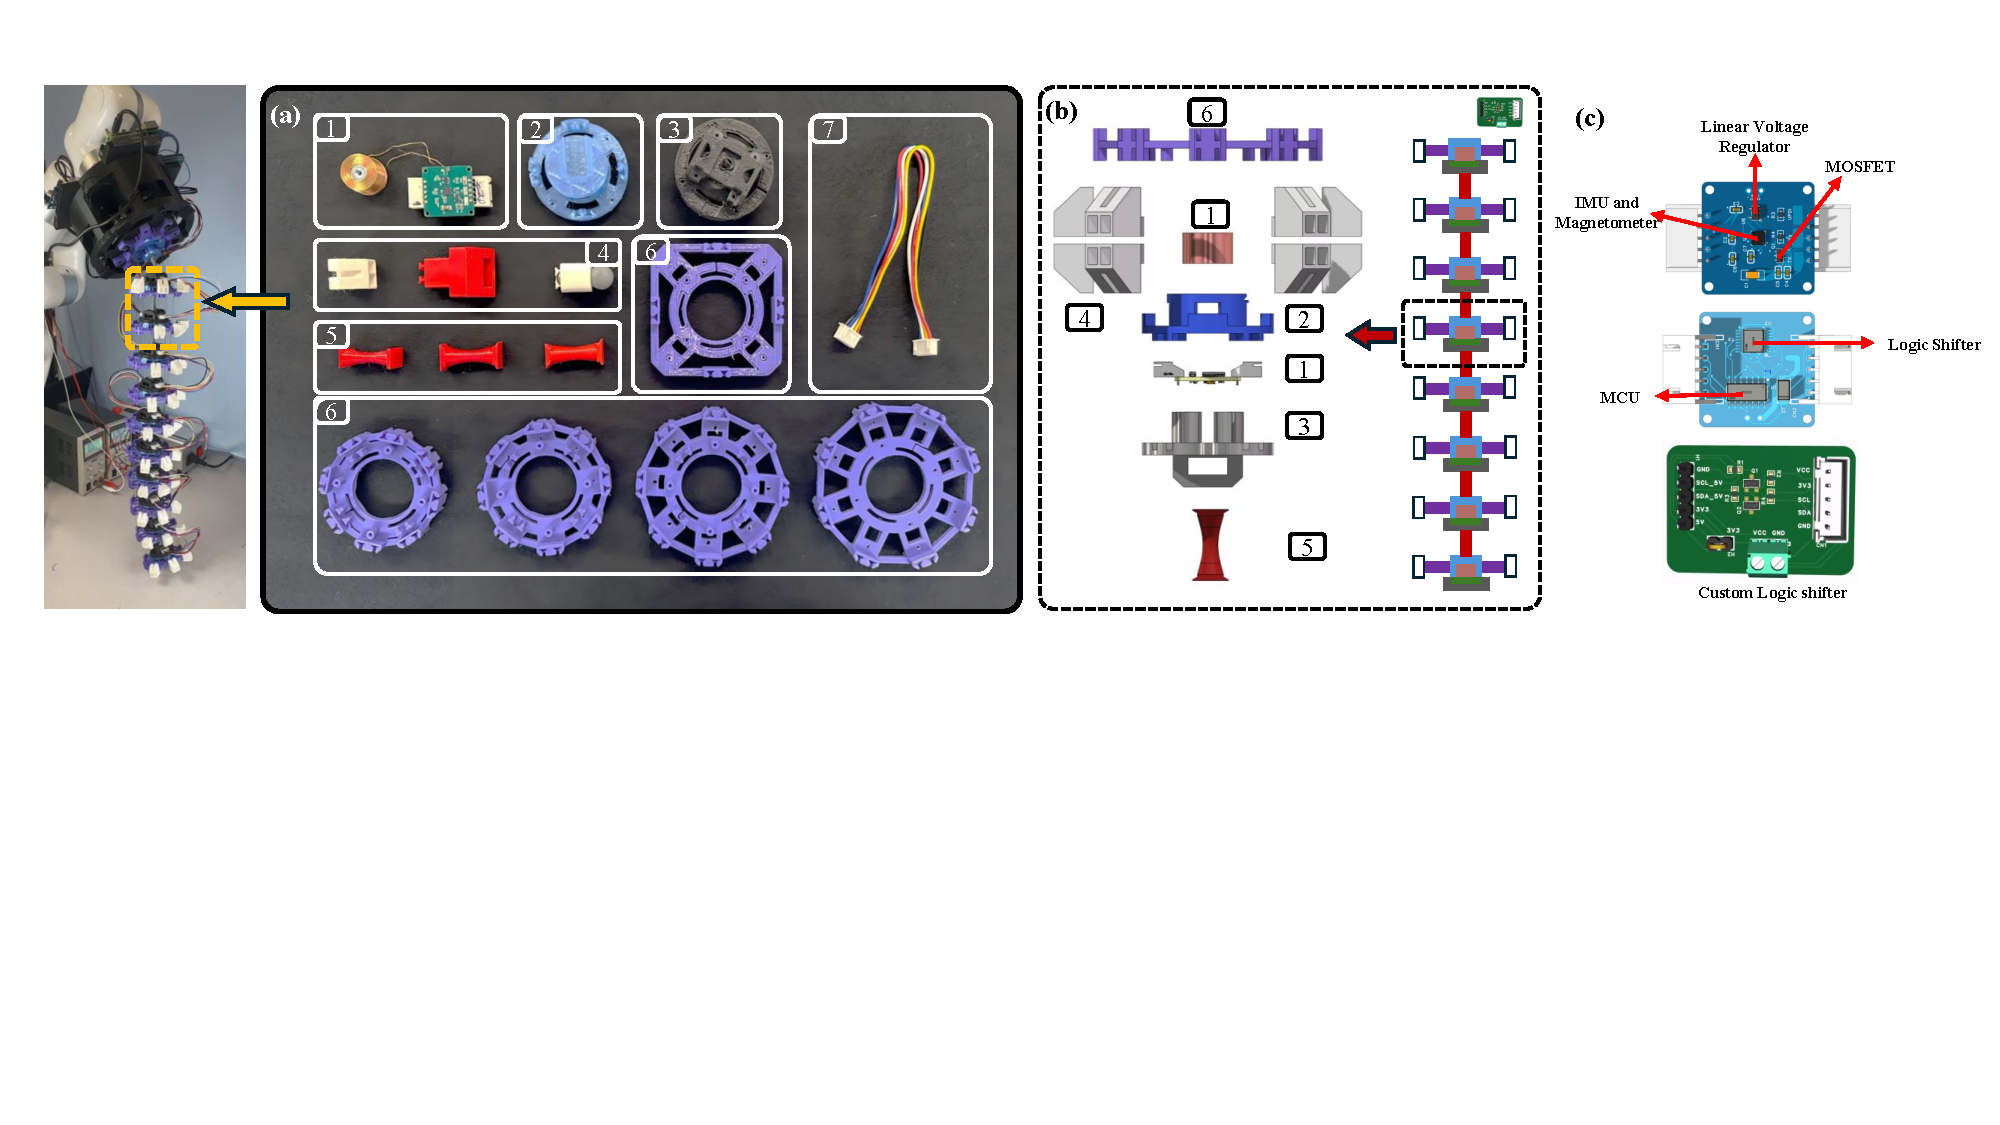
\includegraphics[width=\textwidth]{figs/limb/Fig2_v3.pdf}
    \caption{Overview of the plug-and-play components used to assemble the proposed self-sensing modular continuum robotic platform, including the 3D-printed structural parts and custom electronics. (a) Photograph of the full component set. Numbered parts include (1) sensing module, (2) sensor carrier, (3) cap, (4) stopper insert, (5) flexible joint, (6) limb modules in different sizes, and (7) wiring harness. (b) Exploded view of a single module and its integration into a multi-segment assembly. (c) Custom sensing boards used in each module. The electronics integrate the IMU, magnetometer, voltage regulation, switching, and microcontroller components required for onboard self-sensing.}
    \label{fig:structure}
\end{figure*}

In each segment, a custom printed circuit board (PCB) is embedded to sense the magnetic field generated by the coil in a nearby segment. Each PCB includes a microcontroller (ATTiny3224), a 9-DoF IMU with integrated magnetometer (ICM-20948), a linear drop-out regulator (TPS72118DBVT), a logic shifter (SN74AXC4T774), as well as a diode and an N-channel MOSFET to control the coil. The coils used in the segments are cylindrical, with height 12~mm and diameter 19~mm, wound using 27~AWG wire.

The microcontroller on each PCB acts as a bridge that relays SPI communication to the IMU and I\textsuperscript{2}C communication to an Arduino Mega, which in turn transfers sensor data and coil-control commands to a Raspberry Pi used for inference. Each PCB is daisy chained using JST XH 5-pin connectors carrying both power and communication lines.

Because the IMU operates on 1.8~V logic while the rest of the circuit operates on 3.3~V, a logic shifter is required for communication between these devices. In addition, the Arduino Mega operates at 5~V logic, so a separate custom logic shifter board based on BSS138 NMOS transistors is used to interface the Arduino with the onboard microcontrollers. The sensing boards are shown in Fig.~\ref{fig:structure}(c).

\subsection{Joint Design and Bending Stiffness Characterization}

The modular nature of the design enables the use of joints made from a wide variety of materials and longitudinal and cross-sectional form factors to balance local bending, axial, and torsional stiffness. In this initial study, 3D-printed TPU joints with a simple hourglass-like shape were used, whose stiffness is dictated largely by the minimum neck diameter. As shown in Fig.~\ref{fig:overall}, joints of varying neck diameters can be combined to produce shapes with non-uniform curvature.

The bending stiffness of the joints connecting adjacent rigid segments was estimated using finite-element studies performed in ANSYS Mechanical. Mechanical properties of the TPU joints were determined based on uniaxial tension testing using specimens and procedures comparable to ASTM Standard D412 ~\cite{ASTMD412-2021}. For neck diameters ranging from 3 to 7~mm, a single robot segment was analyzed using a three-dimensional, static, and geometrically nonlinear model subjected to a 30-degree bend angle on one end and a fixed boundary condition on the other.

The reaction moment \(M\) at the fixed end was determined at every three degrees of bend angle \(\theta\). The bending or rotational stiffness of the joint, denoted by \(k\), was determined by fitting a linear relationship between reaction moment and bend angle according to
\begin{equation}
    M = k\theta.
    \label{eq:stiff coef}
\end{equation}

\begin{figure}[!t]
\centering
    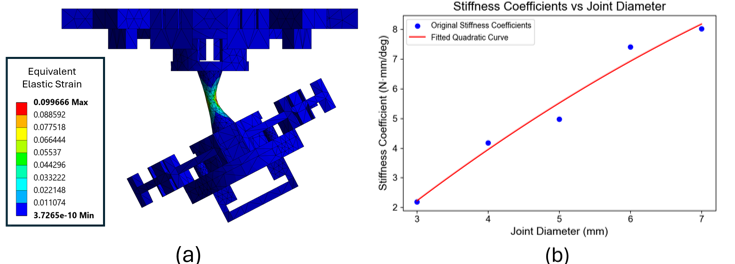
\includegraphics[width=\columnwidth]{figs/limb/image.png}
    \caption{(a) Exemplar strain contours of the finite-element studies. (b) Bending stiffness of joints with varying minimum diameters.}
    \label{fig:fea}
\end{figure}

An exemplar deformed shape and strain contour of a rotated joint segment is shown in Fig.~\ref{fig:fea}, together with the estimated joint bending stiffness for joints ranging from 3 to 7~mm minimum diameter. A quadratic fit of the stiffness trend is shown to illustrate how these and similar analyses could be used in a design setting to determine the exact minimum diameter required to achieve a target bending stiffness for a given application.

This provides a simple and practical way to pre-program the shape response of the robot. By choosing joints with different analytically or numerically precomputed stiffness values, the overall curvature distribution of the robot can be designed in advance while preserving modularity. Future studies may extend this analysis to nonlinear joints whose behavior is shaped by material or geometric design choices to further program the robot shape for different applications.

\section{Pose Estimation}

In contrast to previous continuum-robot self-pose sensing approaches based on distributed strain gauges or embedded cameras and accelerometers ~\cite{fang_design_2023,lilge_continuum_2022,stella_soft_2024}, the system in this chapter uses magnetic sensing by embedding magnetometers and field sources within the robot, similar in spirit to ~\cite{baaij_learning_2023}. Unlike ~\cite{baaij_learning_2023}, which uses permanent magnets, the present design employs electromagnetic coils that can be selectively activated for sensing and deactivated to reduce inter-segment interference.

\begin{figure*}[!t]
    \centering
    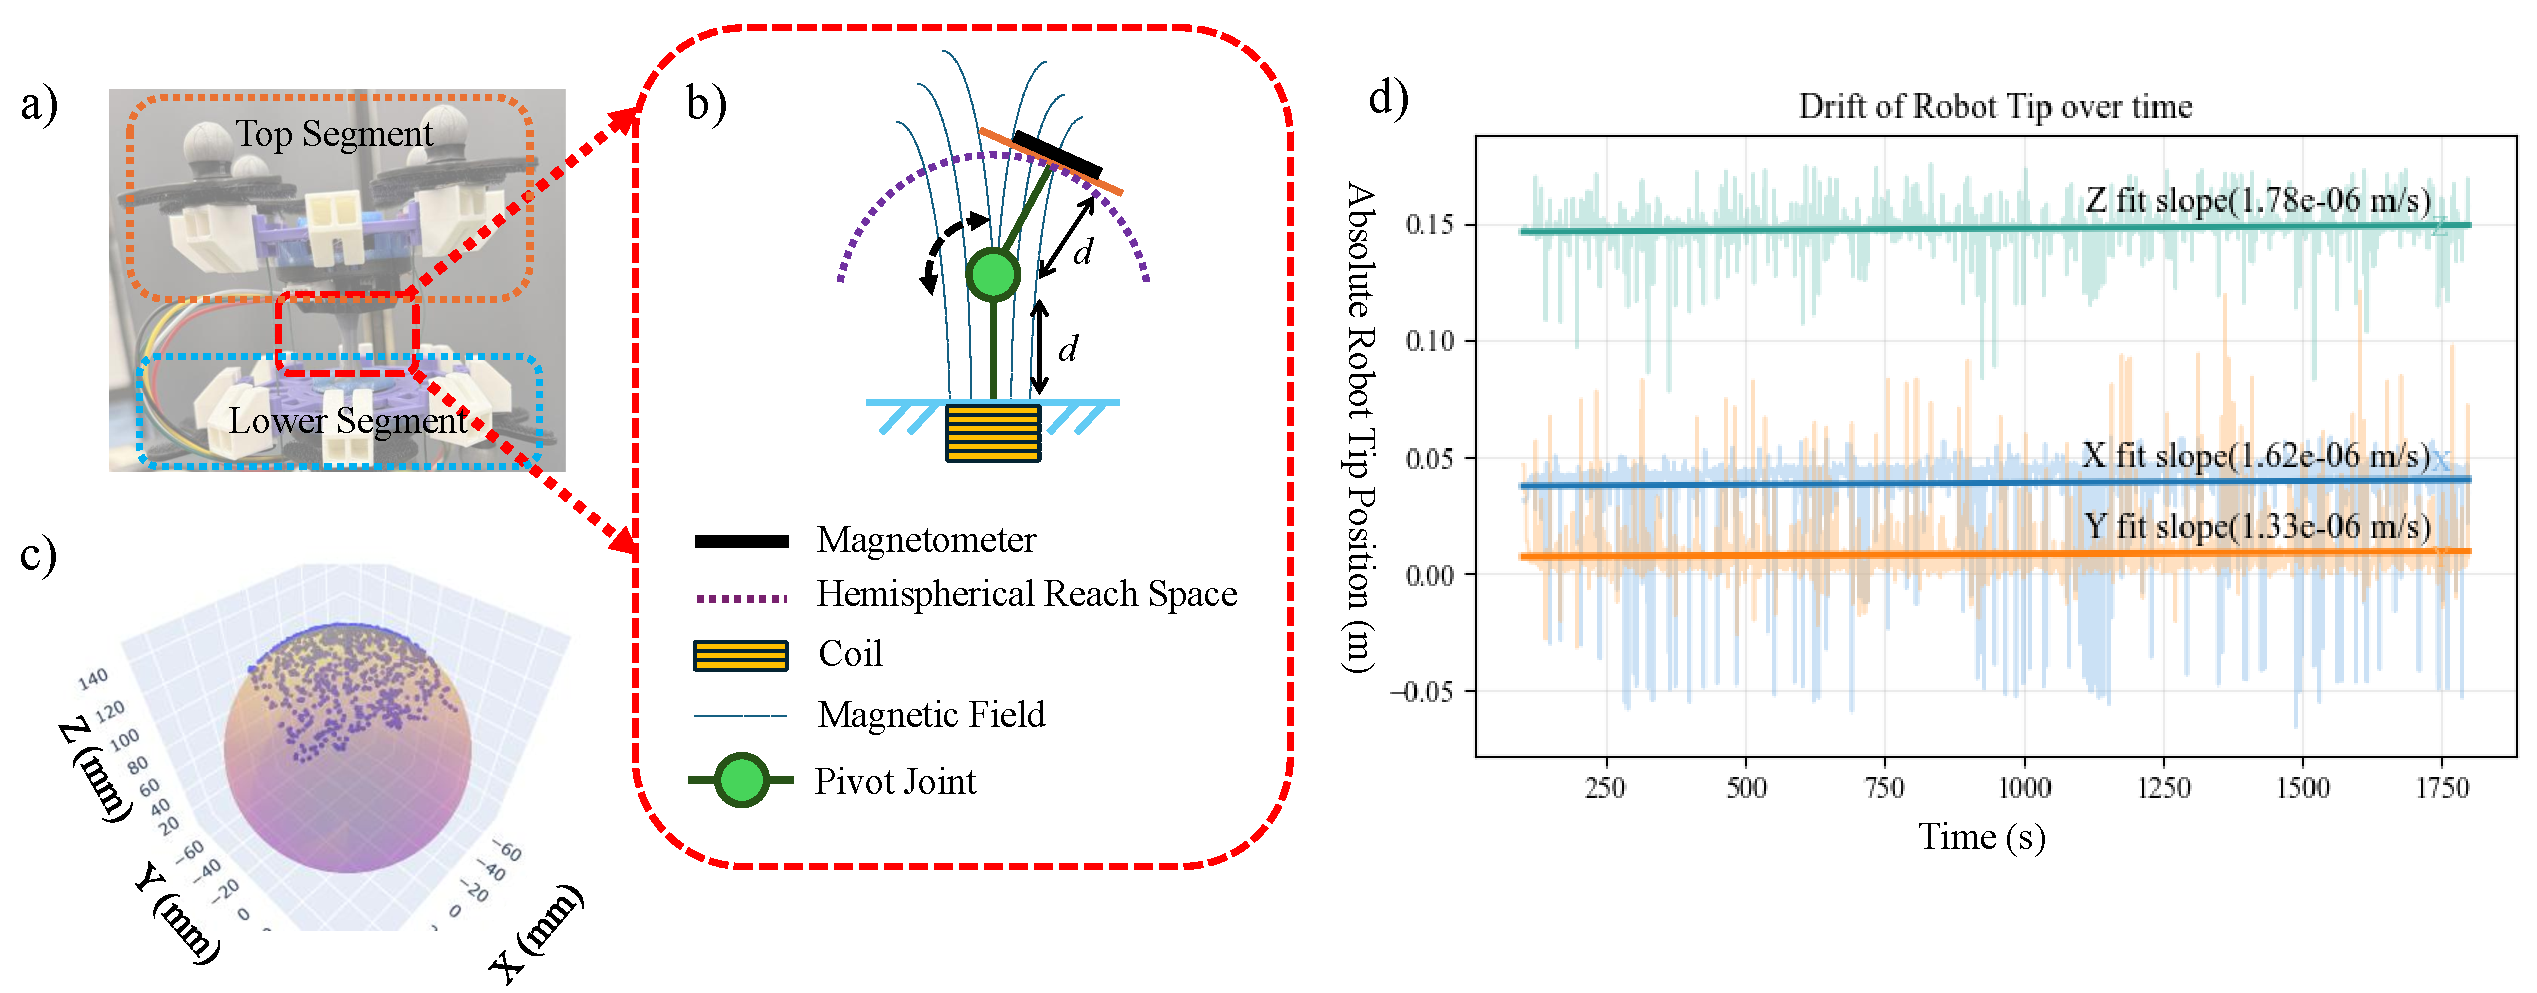
\includegraphics[width=0.9\textwidth]{figs/limb/working_princ.pdf}
    \caption{(a) Example of a pair of segments and the compliant joint between them. In this view, the magnetometer is on the top segment and the coil is on the bottom segment. (b) Schematic of the joint motion. The soft joint is approximated as a rigid hinge with a fixed rotation axis at the joint center and minimal compression, resulting in a dome-like reachable workspace. (c) Motion-capture data of tip positions from one run (500 waypoints), showing that tip positions lie on a hemisphere with 0.523~mm RMSE. (d) Drift test in which the robot is held in a stationary pose for 26 minutes, showing negligible drift.}
    \label{fig:working_principle}
\end{figure*}

The pose-estimation method maps magnetometer measurements in an actively generated magnetic field to relative joint position. As illustrated in Fig.~\ref{fig:working_principle}(b), when adjacent segments bend about a compliant joint, the magnetometer in one segment measures the field produced by the coil embedded in its neighbor. Two assumptions are used. First, the joints maintain a fixed arc length, with bending as the dominant deformation mode. Second, the joints pivot about their geometric center during bending. Together, these assumptions constrain inter-segment motion to a dome-like or hemispherical manifold. The joint design is intended to enforce these conditions, and Fig.~\ref{fig:working_principle}(c) empirically supports their validity.

Under these constraints, the relative position between neighboring segments can be inferred from magnetic field measurements. Because each pair of adjacent segments is treated independently, the sensing method is modular and scales naturally to robots with an arbitrary number of segments.

\subsection{Data Collection}

Training and calibration data for the magnetic-to-position mapping were collected using a two-segment setup. In each run, the lower segment was rigidly mounted to a fixed base to provide a stationary reference frame, while the upper segment was connected through a compliant joint and allowed to rotate freely under tendon actuation. A diagram of the setup is shown in Fig.~\ref{fig:working_principle}(a).

During data collection, randomized wobble motions were executed over the reachable workspace of the joint. The procedure begins by moving all four motors \(\mathcal{I}=\{M_1,M_2,M_3,M_4\}\) to their center positions \(\{c_i\}\). For each waypoint \(k\), two values \((x_k,y_k)\) are sampled uniformly at random from the square \([-1,1]\times[-1,1]\). These values are scaled by an amplitude \(A\) and used to generate target motor commands as symmetric offsets about the motor centers. The resulting commands are clipped to the valid range \([0,4095]\), and the motors are moved to those target positions.

Once the robot reaches the waypoint, the coil is kept \emph{off} and the ambient magnetic bias \(\mathbf{b}_k\) is estimated by averaging a short burst of sensor samples. The coil is then turned \emph{on}, and a second burst of sensor readings is recorded. Finally, the system logs the waypoint index, sampled inputs, motor state, ambient bias, and coil-on readings before moving to the next waypoint. After every 500 waypoints, the system pauses for a cooldown period.

Although the coils are manufacturer matched, small coil-to-coil variations remain. To promote generalization across segments, the roles of the segments were cyclically permuted across runs. After each run, the previously actuated upper segment became the fixed lower segment, and a new segment was introduced as the actuated upper segment. Across all runs, data were collected over approximately \(10^4\) positions and roughly \(10^5\) sensor samples.

To mitigate errors caused by tendon slack, commanded motor positions were not used as ground truth. Instead, accelerometer measurements recorded concurrently with the magnetometer data were used to recover the corresponding 3D ground-truth pose for each waypoint. During each measurement burst the joint is held stationary, so the accelerometer measures gravity alone. Because gravity is perpendicular to the ground plane, this constraint can be used to infer the ground-truth joint pose.

Since the reachable movement space of a joint is assumed to lie on a hemisphere, the joint position is represented using an azimuth angle \(\theta\) and a colatitude angle \(\lambda\). For each sample, let the measured acceleration in the sensor frame be
\begin{equation}
    \mathbf a_b =
        \begin{bmatrix}
        a_{x,b}, 
        a_{y,b}, 
        a_{z,b}
        \end{bmatrix}^T .
\end{equation}
A world-aligned right-handed frame with axes \((X,Y,Z)=(\text{West},\text{North},\text{Out})\) is used, while the sensor axes are mounted as \((x,y,z)=(\text{West},\text{South},\text{Inside})\). The acceleration in the world frame is then defined as
\begin{equation}
    \mathbf a=
        \begin{bmatrix}
        a_x\\
        a_y\\
        a_z
        \end{bmatrix}
        =
        \begin{bmatrix}
        1&0&0\\
        0&-1&0\\
        0&0&-1
        \end{bmatrix}
        \mathbf a_b .
\end{equation}
Since the joint angles depend only on direction, the gravity vector is normalized:
\begin{equation}
    \hat{\mathbf r}=\mathbf a/\|\mathbf a\|_2 =
        \begin{bmatrix}
        r_x, 
        r_y,
        r_z
        \end{bmatrix}^T .
\end{equation}
The colatitude \(\lambda\), measured from the \(+Z\) axis, is then
\begin{equation}
\lambda=\arccos\!\Big(\mathrm{clip}\big(r_z,-1,1\big)\Big),
\end{equation}
and the azimuth \(\theta\), with \(\theta=0\) along North (\(+Y\)) and increasing toward West (\(+X\)), is
\begin{equation}
\theta=\operatorname{atan2}\!\big(r_x,\,r_y\big),
\end{equation}
where \(\theta \in [-\pi,\pi)\).

\subsection{Setup and Training}

To represent the joint pose in a form that avoids discontinuities caused by azimuth wrapping, the angles \((\theta,\lambda)\) are transformed into a 3D direction vector
\begin{equation}
    \mathbf d(\theta,\lambda)=
    \begin{bmatrix}
    \sin\lambda \,\cos\theta\\[4pt]
    \sin\lambda \,\sin\theta\\[4pt]
    \cos\lambda
    \end{bmatrix}.
\end{equation}
This direction vector points from the virtual pivot of the joint to a point on the hemispherical reachable workspace and is used as the target quantity in pose estimation.

The pose-estimation pipeline uses a compact neural network to map normalized magnetometer readings to the corresponding direction vector. Since all segments use identical manufacturer-matched coils, a single joint-level model is trained once over one joint's reachable workspace and then reused across all joints. This greatly reduces the effort required to support different robot configurations and preserves the modularity of the sensing framework.

For training, the collected data from different coils were randomized and split into training and holdout sets. The network parameters were then optimized offline, after which the trained model was exported for deployment. Here the emphasis of this chapter is not on the model architecture itself, but on the modular sensing principle and its integration with the reconfigurable continuum robot hardware.

For real-time inference, the trained model is deployed in ONNX format on a Raspberry Pi~5 running ROS2 Humble in Docker. An Arduino Mega acts as a communication bridge between the magnetometers and the Raspberry Pi.

To minimize magnetic interference between joints in the full robot, only one coil is turned on at any time, and the neighboring segment's magnetometer is sampled sequentially. The inference sampling procedure runs continuously. At the start of each cycle, all coils on the \(N\) bridges are turned \emph{off}. The bridge to sample is selected sequentially as
\begin{equation}
    j = (\texttt{cycle} \bmod N) + 1,
\end{equation}
so that \(j\) cycles through \(1,\dots,N\).

With all coils off, the system waits for an ambient settling time and then reads the IMU from bridge \(j\). The magnetometer vector from this reading is used as the ambient magnetic bias \(\mathbf b_j\). After a short delay, the coil associated with bridge \((j-1)\) is turned \emph{on}, the system waits for the coil-field settling time, and the IMU on bridge \(j\) is read again. The raw magnetometer vector \(\mathbf m_j^{\text{raw}}\) is then debiased using
\begin{equation}
    \mathbf{m}^{\text{deb}}_j = \mathbf{m}^{\text{raw}}_j - \mathbf{b}_j.
\end{equation}
The debiased reading is stored in the sequential array, and once all joints have been sampled the full array is transmitted for pose inference. Finally, the active coil is turned off and the cycle repeats. Including coil settling time and communication overhead, sampling a single joint takes approximately 80~ms, and the full-robot pose-estimation rate is approximately 1.2~Hz.

For evaluation, an OptiTrack Motive motion-capture system was used to capture the position of the robot during deformation as ground truth in the pose-estimation studies.

\subsection{Estimation Results}

\begin{figure*}[!t]
    \centering
    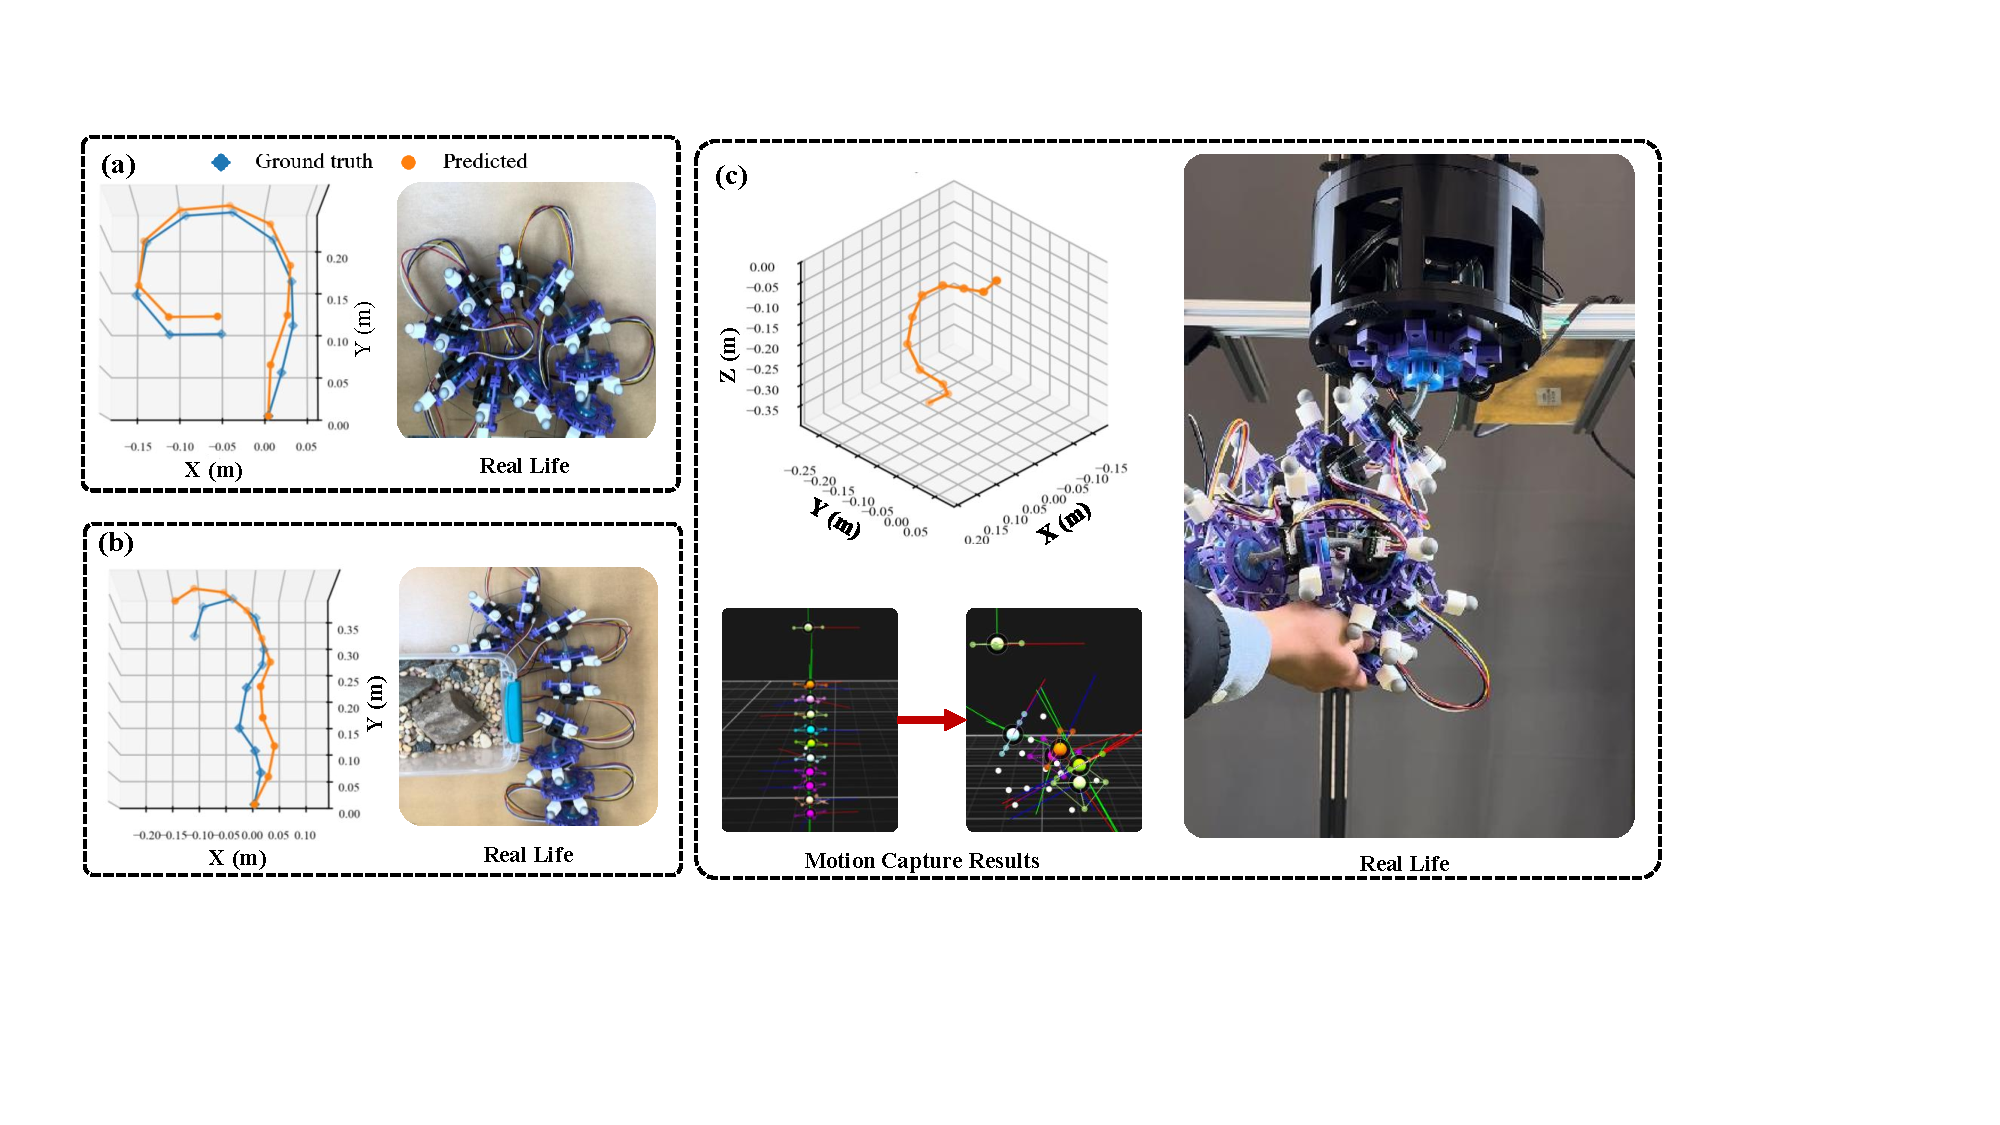
\includegraphics[width=0.95\textwidth]{figs/limb/figure_1_iros_croppedv3.pdf}
    \caption{Pose-estimation results in three scenarios. (a) Scenario 1: the robot moves freely without restriction. The computed RMSE between prediction and ground truth is 0.025483~m. (b) Scenario 2: the robot motion is blocked by a box of rocks. The computed RMSE is 0.0395~m. (c) Scenario 3: the robot is manipulated by hand. In this scenario the motion-capture system failed to track the reflective markers, so no ground truth is available; however, the pose-estimation method still outputs a qualitatively reasonable result under large deformation.}
    \label{fig:pose_estimate_results}
\end{figure*}

Three scenarios were used to evaluate and validate the pose-estimation scheme: (1) unobstructed planar motion, (2) impeded planar motion, and (3) manual 3D manipulation to arbitrary shapes.

In the first scenario, the robot was laid on the ground and allowed to move freely without obstructions. A single tendon was actuated, and the behavior of the pose-estimation scheme was evaluated as the robot curled up. This is the simplest test of the estimator without external influences. The setup and results are shown in Fig.~\ref{fig:pose_estimate_results}(a). The computed RMSE between the estimated and measured positions was 0.025483~m.

In the second scenario, the robot was again placed on the ground, but its motion was impeded by a box of rocks. A single tendon was actuated and the pose estimator was evaluated as the robot deformed under obstacle contact forces. This test probes robustness to unmodeled disturbances in a nominally planar setting. The setup and results are shown in Fig.~\ref{fig:pose_estimate_results}(b), with a computed RMSE of 0.0395~m.

In the third scenario, the robot was suspended vertically and manually manipulated by hand to bend and curl in 3D. Self-occlusion during this motion prevented the motion-capture system from reliably tracking markers, so no usable ground truth was available. Nevertheless, the sensing pipeline still produced pose estimates that appeared qualitatively accurate by visual inspection, as shown in Fig.~\ref{fig:pose_estimate_results}(c).

Overall, these results show that the proposed onboard magnetic sensing method can recover both local inter-segment positions and the global body configuration of the robot across a range of motions. The method also remains usable in contact-rich and partially unstructured settings where external tracking becomes unreliable or unavailable.

\section{Application Demonstrations}

To evaluate the practical versatility of the proposed design, the robot was configured with different combinations of limb, joint, and stopper modules and tested in representative manipulation tasks. These experiments are intended to demonstrate the reconfigurability of the platform and its ability to adapt to different task requirements. Representative results are shown in Fig.~\ref{fig:demo}.

\begin{figure}[!t]
\centering
    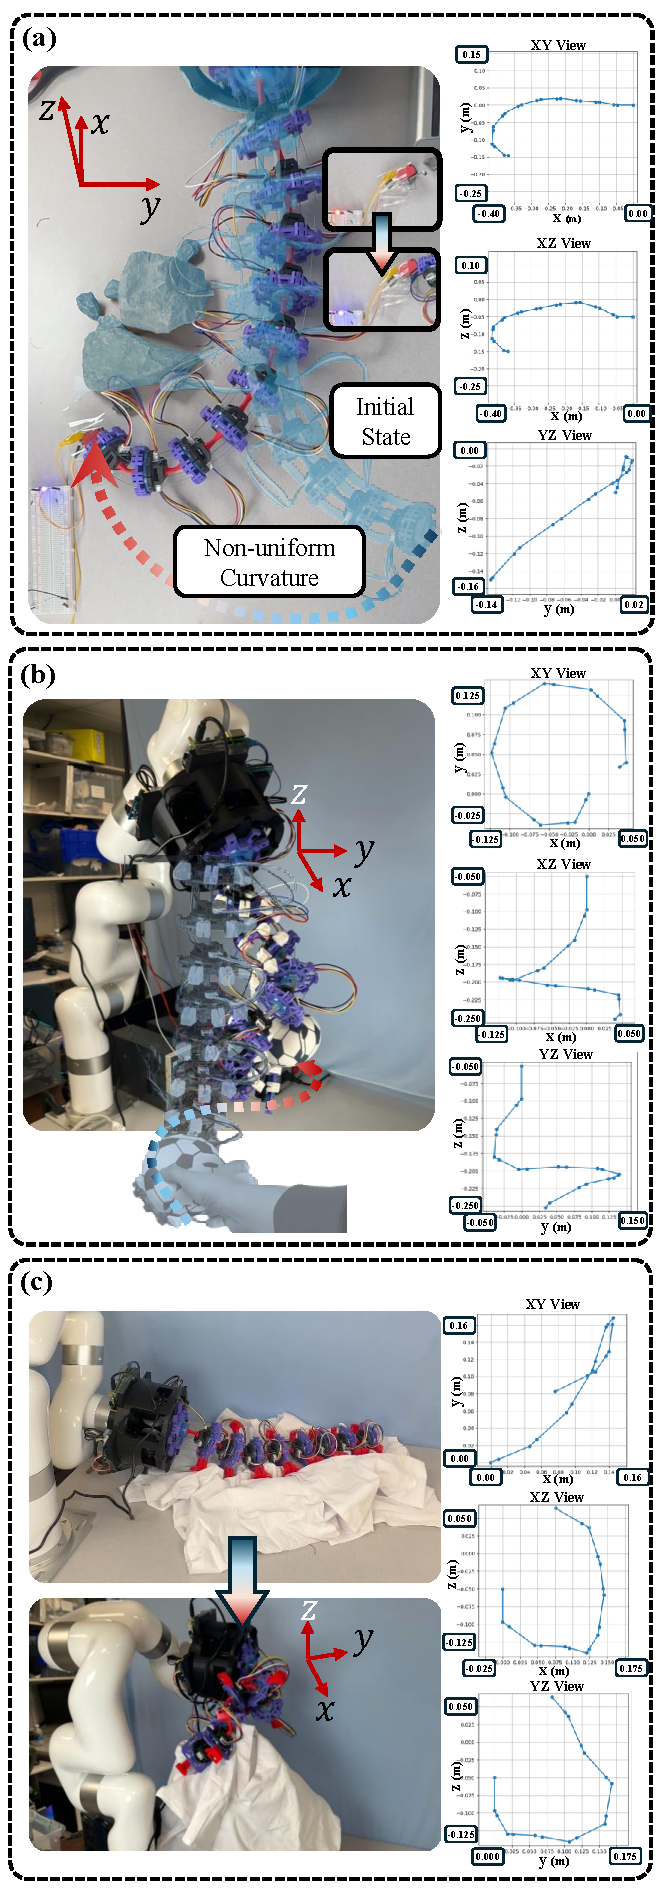
\includegraphics[width=0.43\columnwidth]{figs/limb/iros-26-fig6.pdf}
    \caption{Demonstrations of the modular continuum robotic platform with corresponding pose estimates. (a) Variable-stiffness joints are used to traverse an obstacle and contact a target. (b) Stoppers with softer, higher-friction surfaces are added to enable grasping of a soft spherical object. (c) Alternative limb and ring modules are used to grasp a flexible sheet or cloth.}
    \label{fig:demo}
\end{figure}

First, as shown in Fig.~\ref{fig:demo}(a), limbs with different effective lengths and flexible joints with different bending stiffnesses were combined to promote non-uniform curvature under tendon actuation. The selected lengths and stiffnesses enabled the robot to bend around an obstacle and reach a target position for a switch.

Second, a spherical grasping task was performed using TPU stopper modules coated with Eco-Flex 00-30, as shown in Fig.~\ref{fig:demo}(b). This configuration provided both compliant contact and increased surface friction, allowing the robot to stably envelop and grasp a sphere with a diameter of approximately 12~cm. The result demonstrates how simply replacing contact modules can substantially improve grasping performance for smooth curved objects.

Third, square limb modules were combined with stopper inserts designed to provide larger gripping force for cloth grasping, as shown in Fig.~\ref{fig:demo}(c). Compared with the previous configuration, this setup generated stronger local contact forces and was better suited for handling deformable objects. This further demonstrates that the same platform can be rapidly reconfigured to accommodate different object geometries and contact conditions.

In all three tasks, the proposed pose-estimation method was used to predict the robot shape during operation. The results show that the method can effectively estimate both the relative positions between neighboring segments and the overall body configuration while maintaining good performance during real contact-rich interactions. Taken together, these demonstrations validate the effectiveness and generality of the proposed self-sensing modular continuum robotic platform in diverse manipulation tasks.

\section{Chapter Summary}

This chapter presented an in-situ self-pose estimation framework for modular continuum robots. The proposed platform combines mechanically reconfigurable continuum segments with onboard magnetic sensing, allowing both robot morphology and sensing capability to be assembled in a modular manner. Through interchangeable joints with precomputed bending stiffness, the robot can be configured to realize different curvature distributions and task-specific mechanical behaviors.

This chapter also demonstrated that self-contained pose estimation can be achieved without external tracking during operation. By inferring relative inter-segment position from local magnetic measurements and combining these estimates along the robot body, the method provides a practical way to reconstruct robot shape across different configurations. Experimental results in multiple motion scenarios and contact-rich manipulation tasks validated both the reconfigurability of the hardware and the effectiveness of the sensing approach. These results show that modular design and embedded proprioception are complementary building blocks for more adaptable and deployable continuum robotic systems.
